\documentclass[12pt, twoside]{article}
\usepackage[letterpaper, margin=1in, headsep=0.5in]{geometry}
\usepackage[english]{babel}
\usepackage[utf8]{inputenc}
\usepackage{amsmath}
\usepackage{amsfonts}
\usepackage{amssymb}
\usepackage{tikz}
\usetikzlibrary{quotes, angles}
\usepackage{graphicx}
\usepackage{enumitem}
\usepackage{multicol}
\usepackage{hyperref}

\newif\ifmeta
\metatrue %print standards and topics tags

\title{IB Mathematics}
\author{Chris Huson}
\date{September 2021}

\usepackage{fancyhdr}
\pagestyle{fancy}
\fancyhf{}
\renewcommand{\headrulewidth}{0pt} % disable the underline of the header
\raggedbottom


\fancyhead[LE]{\thepage}
\fancyhead[RO]{\thepage \\ Name: \hspace{4cm} \,\\}
\fancyhead[LO]{BECA / IB Math 01-Linear functions\\* 20 January 2022}

\begin{document}

\subsubsection*{PreQuiz: I can model arithmetic sequences}
Arithmetic sequences\\[0.25cm]
Terms: $u_n=u_1 + d(n-1)$\\[0.25cm]
Sum: $\displaystyle S_n= \frac{n}{2}(u_1 + u_n)$\\[0.25cm]

\begin{enumerate}
\item In an arithmetic sequence the first term is $-5$ and the fourth term is 4.
  \begin{enumerate}[itemsep=2cm]
    \item Find the common difference $d$.
    \item Find the eighth term, $u_{8}$.\vspace{1cm}
    \item Find the sum of the first eight terms.
  \end{enumerate} \vspace{2cm}

\item The second term of an arithmetic sequence is 22 and the seventh term is 2.
  \begin{enumerate}[itemsep=2cm]
    \item Find the common difference $d$.
    \item Find the first term, $u_{1}$.
    \item Find the sum of the first seven terms.
  \end{enumerate} \vspace{2cm}

\newpage
\item The rate on a credit card is $18\%$ per annum. Find the total amount due on a \$650 purchase after one month (principal and interest). \vspace{3cm}

\item Robert takes out a 5 month loan to purchase and repair a used car for resale. The principal amount is 12,000 euros and interest rate is $9.50\%$ per annum. Find the interest Robert pays. \vspace{3cm}

\item The height of a plant $h$ in centimeters over a period of time $t$ measured in weeks is shown in the table. \hfill [3]
\begin{enumerate}
  \item Plot the data as points on the grid.
  \item Draw a line of best fit on the graph.
\end{enumerate}
  \begin{center} 
  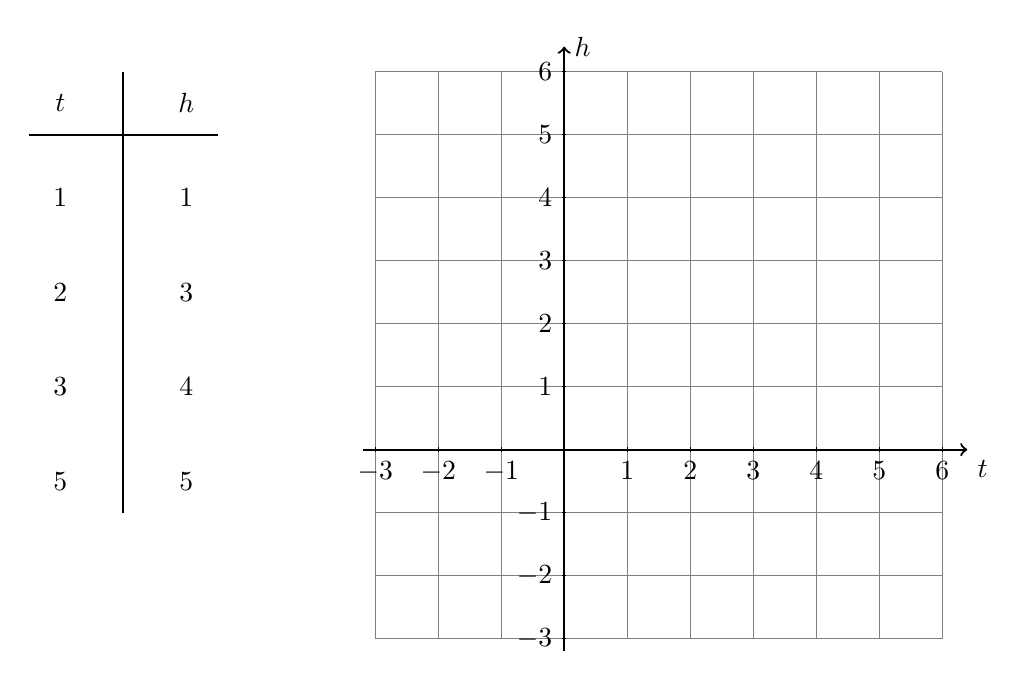
\begin{tikzpicture}[scale=0.8]
    \draw [help lines] (-3,-3) grid (6,6);
    \draw [thick, ->] (-3.2,0) -- (6.4,0) node [below right] {$t$};
    \draw [thick, ->] (0,-3.2)--(0,6.4) node [right] {$h$};
    \foreach \x in {-3,-2,-1,1,2,3,4,5,6} \draw (\x cm,1pt) -- (\x cm,-1pt) node[anchor=north] {$\x$};
    \foreach \y in {-3,-2,-1,1,2,3,4,5,6} \draw (1pt,\y cm) -- (-1pt,\y cm) node[anchor=east] {$\y$};

    \draw [thick] (-7,-1) -- (-7,6);
    \draw [thick] (-8.5,5) -- (-5.5,5);
    \node at (-8,5.5){$t$}; \node at (-6,5.5){$h$};

    \node at (-8,4){$1$}; \node at (-6,4){$1$};
    \node at (-8,2.5){$2$}; \node at (-6,2.5){$3$};
    \node at (-8,1){$3$}; \node at (-6,1){$4$};
    \node at (-8,-0.5){$5$}; \node at (-6,-0.5){$5$};
  \end{tikzpicture}
  \end{center}

\end{enumerate}
\end{document}